\section{Preprocesamiento de datos}

\subsection{Exploración de datos}
Se realizaron ciertas tareas de exploración de datos 
sobre el FLAME dataset, para lo cual el enfoque fueron las imágenes de entrenamiento
y prueba de las categorías \textbf{Fire} y \textbf{No\_Fire}. A continuación, se muestra 
un resumen de los principales hallazgos:
\begin{enumerate}
    \item \textbf{Distribución de imágenes:}
      \begin{enumerate}
          \item \textbf{Entrenamiento:}
          \begin{itemize}
              \item \textbf{No\_Fire:} 14\,357 imágenes (\(\approx 36.45\%\))
              \item \textbf{Fire:} 25\,027 imágenes (\(\approx 63.55\%\))
          \end{itemize}
          \item \textbf{Prueba:}
          \begin{itemize}
              \item \textbf{No\_Fire:} 5\,137 imágenes (\(\approx 59.61\%\))
              \item \textbf{Fire:} 3\,480 imágenes (\(\approx 40.39\%\))
          \end{itemize}
      \end{enumerate}
      Se observa un desbalance en el conjunto de entrenamiento, donde la categoría \textbf{Fire} 
      predomina.
      
    \item \textbf{Formato y dimensiones:}  
      Todas las imágenes se encuentran en formato JPEG y poseen dimensiones uniformes. 
    
    \item \textbf{Análisis de color:}  
      Se realizó un estudio de los histogramas de color para identificar patrones en las distribuciones de intensidades:
      \begin{itemize}
          \item Las imágenes de la categoría \textbf{Fire} muestran picos de intensidad en el canal rojo, 
          lo cual es coherente con la presencia de fuego y las altas temperaturas que generan tonos más cálidos.
          \item En contraste, las imágenes de la categoría \textbf{No\_Fire} exhiben distribuciones 
          de color más uniformes o predominio de tonos verdes y azules, lo que sugiere escenas más naturales 
          o ambientes sin fuego. 
      \end{itemize}
      Debajo se muestran algunos histogramas de dichas categorías:
      \begin{figure}[htbp]
        \centering
        \begin{minipage}[b]{0.45\textwidth}
          \centering
          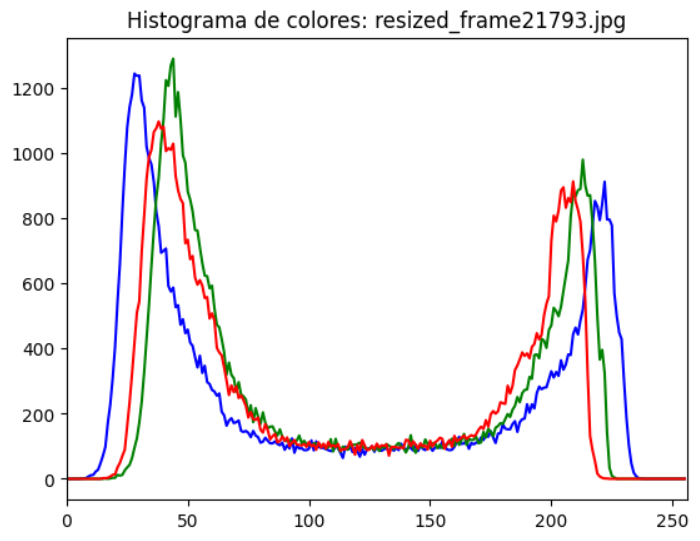
\includegraphics[width=\linewidth]{images/histograma_fire.png}
          \vspace{0.5em}
          \small\textbf{Fire}
        \end{minipage}
        \hfill
        \begin{minipage}[b]{0.45\textwidth}
          \centering
          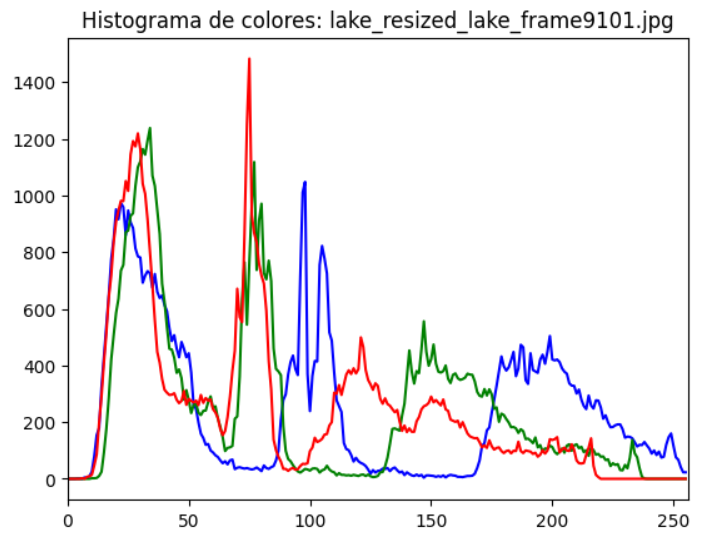
\includegraphics[width=\linewidth]{images/histograma_no_fire.png}
          \vspace{0.5em}
          \small\textbf{No\_Fire}
        \end{minipage}
        \caption{Histogramas de color para las categorías \textbf{Fire} y \textbf{No\_Fire}.}
        \label{fig:histograms}
      \end{figure}

\end{enumerate}

\subsection{Redimensionamiento y Aumento de datos}
Dado que emplearemos modelos preentrenados, se optó por redimensionar todas las imágenes 
a 224x224 píxeles. Para este propósito, se implementó una función que emplea 
el método de remuestreo LANCZOS (óptimo para preservar la calidad). Luego, se guardaron las imágenes
en una estructura de directorios paralela a la original.

Además, durante la etapa de exploración, se observó un desbalance significativo entre las 
dos categorías de los datos de entrenamiento. En particular, la clase \textbf{Fire} contaba con un mayor número 
de imágenes que la clase \textbf{No\_Fire}. 

A fin de abordar este problema y mejorar la capacidad de generalización del modelo, 
se aplicó una técnica de \emph{data augmentation} utilizando la clase \texttt{ImageDataGenerator} de Keras. 
Esta técnica genera nuevas imágenes a partir de las originales aplicando transformaciones aleatorias, 
lo que permite aumentar el número de ejemplos y enriquecer el dataset con variaciones realistas. 
Las transformaciones utilizadas fueron:

\begin{itemize}
    \item \textbf{Rotación:} Se rotó la imagen en un rango de $\pm30^\circ$, ayudando al modelo a 
    reconocer objetos independientemente de su orientación.
    \item \textbf{Desplazamiento:} Se realizaron cambios aleatorios en la posición horizontal y 
    vertical (hasta el 20\% del tamaño), lo que permitió que el modelo sea menos sensible a la 
    ubicación del objeto dentro de la imagen.
    \item \textbf{Cizallamiento (shear):} Se aplicó una deformación de la imagen que simula cambios en la perspectiva, 
    contribuyendo a la robustez del modelo frente a distorsiones.
    \item \textbf{Zoom:} Se efectuó un zoom in/out en un rango del 20\%, generando variaciones en la escala del objeto.
    \item \textbf{Volteo horizontal:} Se invirtió la imagen de forma horizontal, lo cual duplica 
    las variaciones disponibles y es especialmente útil cuando la orientación no afecta la clasificación.
    \item \textbf{Relleno:} Se utilizó el modo de relleno \texttt{'nearest'} para completar los espacios 
    vacíos que puedan generarse durante las transformaciones.
\end{itemize}

Para aplicarlo, se calculó el número de imágenes adicionales necesarias de tal forma que la cantidad de 
imágenes en la clase \textbf{No\_Fire} sea equivalente a la de \textbf{Fire}. Luego, 
el generador aplicó de forma iterativa estas transformaciones a cada imagen de la categoría \textbf{No\_Fire} y se 
guardaron las nuevas imágenes en un directorio específico para datos aumentados. Debajo se muestra un 
ejemplo de una imagen aumentada.

\begin{figure}[htbp]
    \centering
    \begin{minipage}[b]{0.45\textwidth}
      \centering
      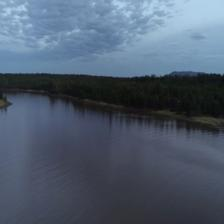
\includegraphics[width=\linewidth]{images/original.jpg}
      \vspace{0.5em}
      \small\textbf{Original}
    \end{minipage}
    \hfill
    \begin{minipage}[b]{0.45\textwidth}
      \centering
      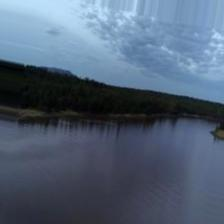
\includegraphics[width=\linewidth]{images/aumentada.jpg}
      \vspace{0.5em}
      \small\textbf{Aumentada}
    \end{minipage}
    \caption{Ejemplo de imagen original y su versión aumentada en la categoría \textbf{No\_Fire}.}
    \label{fig:original_aumentada}
  \end{figure}


